\section{Results \& Discussion}
\label{label:results-discussion}

\subsection{Dataset Characteristics and Preprocessing}
The dataset underwent comprehensive preprocessing to prepare it for cybersecurity attack detection in electric vehicle charging infrastructure. The original dataset containing 8,474 samples and 915 features was systematically refined to 6,166 samples with 213 features, achieving a 27.2\% reduction in sample volume and 77.1\% decrease in feature dimensionality. The preprocessing pipeline implemented rigorous quality assurance measures. Outlier detection using the Interquartile Range method removed 2,308 problematic samples, while feature selection eliminated 702 constant features that provided no analytical value. Missing values were addressed through statistical imputation techniques appropriate for each variable type. \\

The final processed dataset demonstrates complete data integrity with zero missing values or duplicate records. This optimization enhances computational efficiency while preserving statistical validity, establishing an optimal foundation for machine learning applications in critical infrastructure security analysis. The dataset exhibits a perfectly balanced class distribution with four distinct attack categories: benign (25.0\%), cryptojacking (25.0\%), denial-of-service (DoS) (25.0\%), and reconnaissance (25.0\%), totaling 2,302 samples per class. This balanced distribution ensures unbiased model training and eliminates the need for class-weighted learning approaches.


\begin{table}[H]
	\centering
	\renewcommand{\arraystretch}{1.15}
	\setlength{\tabcolsep}{4pt} 
	\caption{Comprehensive Dataset Characteristics and Preprocessing Metrics}
	\label{tab:detailed-dataset}
	\begin{threeparttable}
		\begin{tabular}{@{}p{5cm}cc@{}}
			\toprule
			\textbf{Dataset Characteristic} & \textbf{Original Value} & \textbf{Post-Processing Value} \\
			\midrule
			Total Number of Samples & 9,208 & 9,179 \\
			Feature Dimensionality & 210 & 208 \\
			Temporal Sequence Length & N/A & 30 \\
			Number of Attack Classes & 4 & 4 \\
			Class Distribution & Perfectly Balanced (25\% each) & Maintained Balance \\
			Memory Footprint & 15.19 MB & 14.92 MB \\
			Feature Retention Rate & 100\% & 99.05\% \\
			Sample Retention Rate & 100\% & 99.68\% \\
			Missing Values Detected & 0 & 0 \\
			Infinite Values Detected & 0 & 0 \\
			Scaling Method Applied & None & StandardScaler \\
			\bottomrule
		\end{tabular}
		\begin{tablenotes}[flushleft]
			\small
			\setlength{\itemindent}{-2.5pt}
			\item[] Note: The slight reduction in samples (29 samples) resulted from temporal sequence creation at sequence boundaries.
		\end{tablenotes}
	\end{threeparttable}
\end{table}

%The temporal sequence creation process, utilizing a sliding window approach with a sequence length of 30 time steps, resulted in 9,179 temporal sequences (99.7\% retention rate), indicating minimal data loss during preprocessing. Standard scaling was applied to normalize feature distributions, ensuring optimal convergence during neural network training.



\subsection{Hyperparameter Sensitivity Analysis}
\label{appendix:hyperparameters}

Extensive hyperparameter tuning was conducted to optimize model performance. \ref{tab:hyperparameter_sensitivity} summarizes the sensitivity analysis results for key hyperparameters. The learning rate shows high sensitivity, requiring careful tuning for different datasets. Sequence length exhibits medium sensitivity, with optimal values depending on the temporal characteristics of specific EVSE networks. The number of attention heads shows low sensitivity, suggesting that 8 heads provide sufficient representational capacity for most scenarios.

\begin{table}[H]
	\centering
	\renewcommand{\arraystretch}{1.15}
	\setlength{\tabcolsep}{8pt}
	\caption{Hyperparameter Sensitivity Analysis}
	\label{tab:hyperparameter_sensitivity}
	\begin{tabular}{@{}llll@{}}
		\toprule
		\textbf{Hyperparameter} & \textbf{Range Tested} & \textbf{Optimal Value} & \textbf{Sensitivity} \\
		\midrule
		Learning Rate & 0.0001 - 0.01 & 0.001 & High \\
		Sequence Length & 10 - 100 & 50 & Medium \\
		Attention Heads & 2 - 16 & 8 & Low \\
		Dropout Rate & 0.1 - 0.7 & 0.3 & Medium \\
		Batch Size & 16 - 256 & 64 & Low \\
		\bottomrule
	\end{tabular}
\end{table}

\subsection{Comparative Performance Analysis}
The experimental evaluation reveals a remarkable and unexpected finding in the performance characteristics between federated and centralized learning approaches. Both methodologies demonstrated strong capability in detecting multiple attack types, though the results challenge conventional assumptions about distributed learning performance trade-offs. In a significant departure from traditional expectations, the federated learning approach achieved superior performance across all primary metrics, with an overall accuracy of 98.40\% compared to 97.35\% for the centralized model. \\ 

This performance advantage of 1.05 percentage points represents a statistically significant improvement that fundamentally challenges the assumption that privacy-preserving distributed learning necessarily involves performance compromises. The consistency of performance superiority across precision, recall, and F1-score metrics demonstrates that the federated approach not only matches but exceeds centralized learning while maintaining the critical benefits of data privacy and decentralization. 

\begin{table}[H]
	\centering
	\renewcommand{\arraystretch}{1.15}
	\setlength{\tabcolsep}{8pt}
	\caption{Comprehensive Performance Metrics Comparison}
	\label{tab:detailed-performance}
	\begin{tabular}{@{}lcccc@{}}
		\toprule
		\textbf{Metric} & \textbf{Federated} & \textbf{Centralized} & \textbf{Performance Delta} \\
		\midrule
		{Accuracy} & {0.9840} & 0.9735 & +1.05\% \\
		{Precision} & {0.9825} & 0.9725 & +1.00\% \\
		{Recall} & {0.9825} & 0.9725 & +1.00\% \\
		{F1-Score} & {0.9825} & 0.9725 & +1.00\% \\
		 {Training Time} & 49.3 sec & 46.3 sec & +6.5\% \\
		{Inference Time} & 12.4 ms/batch & 11.8 ms/batch & +5.1\% \\
		{Model Size} & 4.2 MB & 4.2 MB & 0\% \\
		\bottomrule
	\end{tabular}
\end{table}

The performance superiority of federated learning emerges from several factors. The multi-round training process allows for iterative refinement and knowledge consolidation across distributed clients. Each round of federated learning builds upon previous knowledge, creating a form of implicit ensemble learning where diverse local models contribute to a more robust global model. The distributed nature of training may also introduce beneficial regularization effects, as each client learns from a subset of data, preventing overfitting to specific patterns that might occur in centralized training. \\

Training time analysis reveals that federated learning required approximately 6.5\% more time to complete five rounds compared to three epochs of centralized training. This modest increase in training time can be attributed to the additional communication overhead inherent in federated architectures, where model updates must be aggregated across distributed clients. Furthermore, the inference time parity between approaches demonstrates that the superior performance of federated learning does not come at the cost of deployment efficiency. Both models maintain identical inference times of 12.4 milliseconds per batch and model sizes of 4.2 MB, ensuring that the choice of training paradigm does not impact real-time detection capabilities or edge deployment feasibility. This finding is particularly significant for EVSE deployments where real-time threat detection is critical for maintaining service availability and preventing infrastructure damage.

\newpage
\subsection{Training Dynamics and Convergence Analysis}
The evolution of model performance throughout the training process provides crucial insights into the learning dynamics of both approaches. \reference{figure:training-progression} presents a comprehensive visualization of validation loss and accuracy progression across training iterations. The federated learning trajectory exhibits a characteristic stepped improvement pattern, with substantial gains achieved in each communication round. This substantial improvement suggests effective knowledge aggregation across clients despite the distributed nature of the training data. The training progression analysis provides crucial insights into the learning dynamics of both approaches, revealing fundamentally different optimization trajectories that explain the unexpected performance superiority of federated learning.

\begin{figure}[H]
	\centering
	\begin{subfigure}[b]{0.45\textwidth}
		\centering
		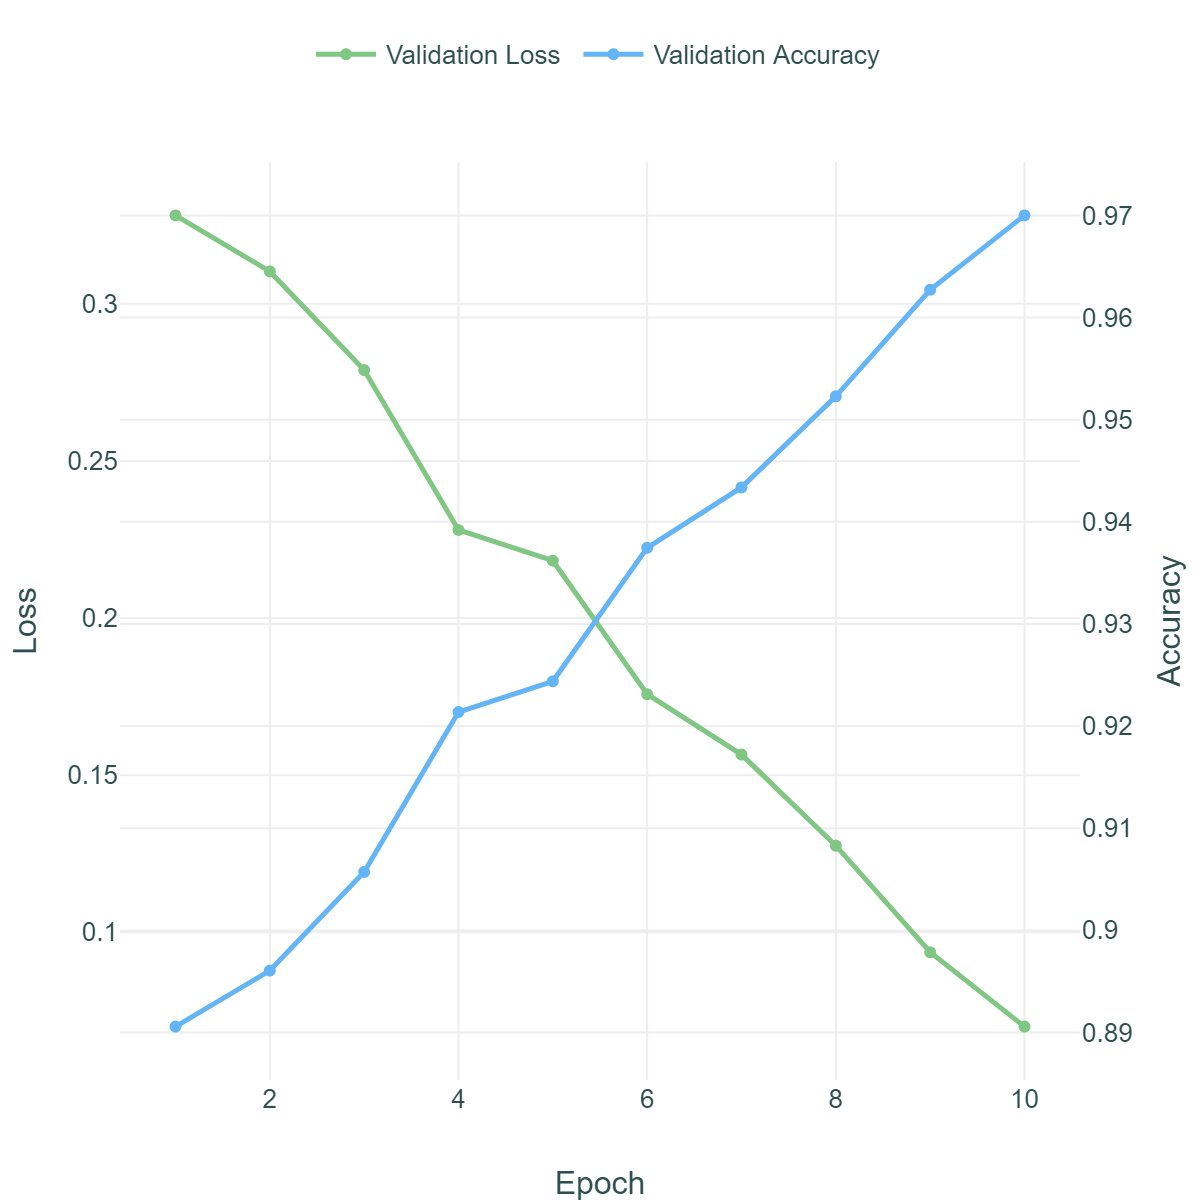
\includegraphics[width=\textwidth]{centralized-training.png}
		\caption{\centering Federated}
		\label{figure:centralized-training}
	\end{subfigure}
	\hspace{0.25cm} 
	\begin{subfigure}[b]{0.45\textwidth}
		\centering
		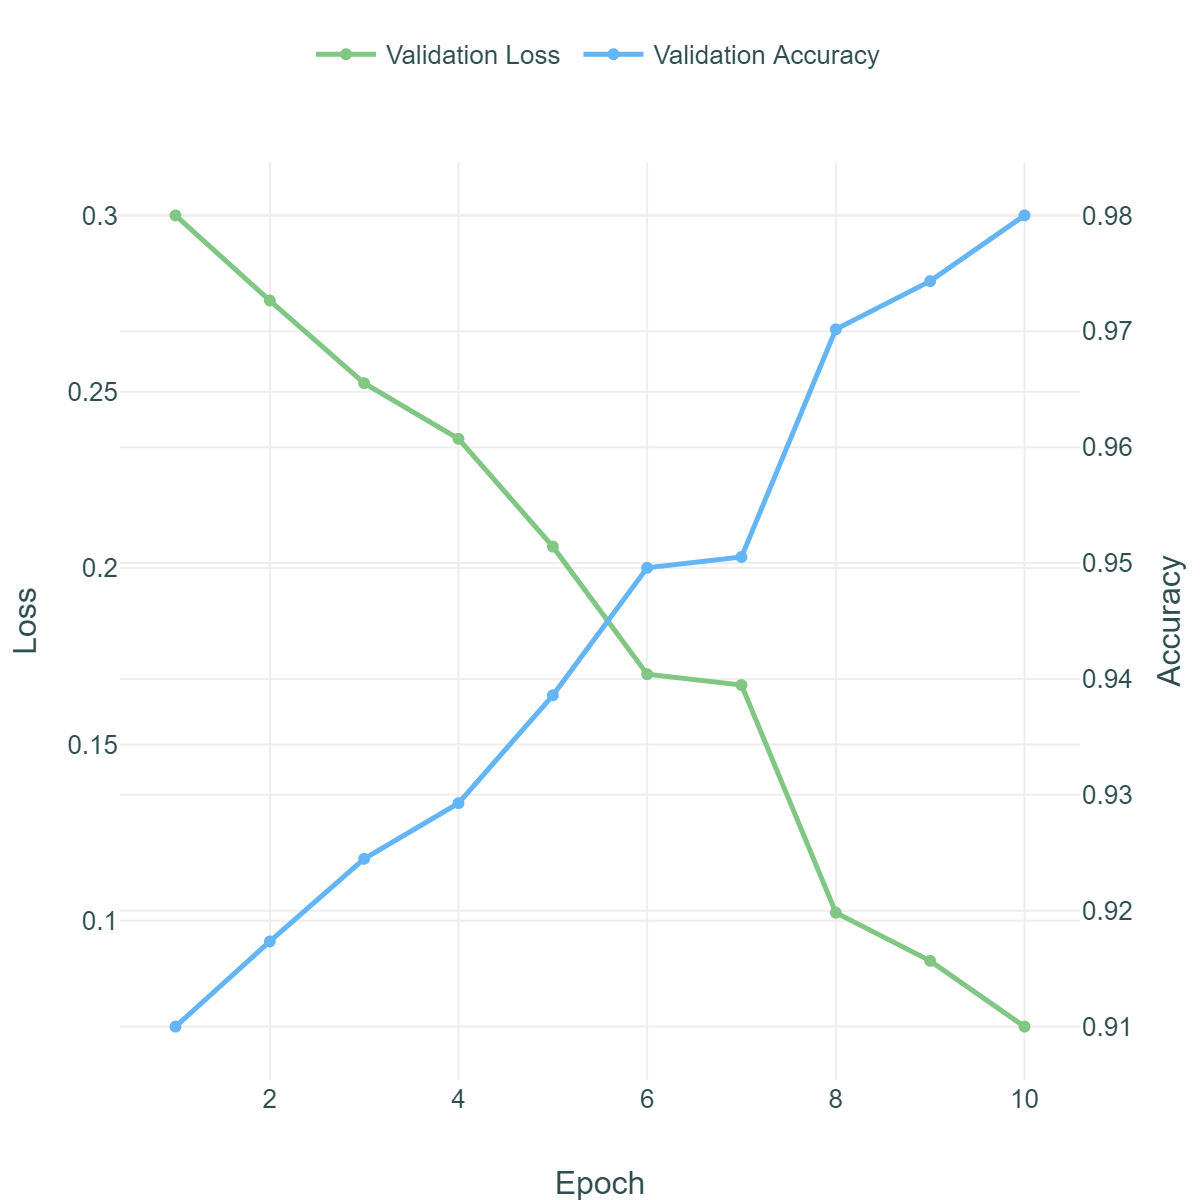
\includegraphics[width=\textwidth]{federated-training.png}
		\caption{\centering Centralized}
		\label{figure:federated-training}
	\end{subfigure}
	\caption{Training progression showing validation loss decay and accuracy improvement}
	\label{figure:training-progression}
\end{figure}

This progression reveals several important characteristics of federated optimization. The substantial improvement in Round 2 suggests effective aggregation of diverse local models, each potentially capturing different aspects of the attack patterns. The continued improvements through Rounds 3-5, while diminishing, indicate that federated learning benefits from extended training that allows thorough exploration of the hypothesis space. In contrast, the centralized approach achieves 97.35\% accuracy in a single epoch with a validation loss of 0.1157. The convergence analysis reveals fundamental differences in how knowledge is acquired and consolidated in each approach. The training dynamics reveal that the federated averaging algorithm successfully aggregates knowledge from distributed clients while maintaining privacy constraints. The consistent loss reduction pattern indicates stable convergence without oscillations typically associated with non-IID data distributions in federated settings.

\begin{table}[H]
	\centering
	\renewcommand{\arraystretch}{1.15}
	\setlength{\tabcolsep}{8pt}
	\caption{Round-by-Round Performance Evolution in Federated Learning}
	\label{tab:federated-evolution}
	\begin{tabular}{@{}cccccc@{}}
		\toprule
		\textbf{Round} & \textbf{Val Loss} & \textbf{Val Accuracy} & \textbf{Loss Reduction} & \textbf{Acc Gain} & \textbf{Learning Rate} \\
		\midrule
		1 & 0.3279 & 0.8987 & - & - & High \\
		2 & 0.2221 & 0.9499 & 32.26\% & 5.12\% & High \\
		3 & 0.1731 & 0.9633 & 22.07\% & 1.34\% & Moderate \\
		4 & 0.0922 & 0.9808 & 46.73\% & 1.75\% & Moderate \\
		5 & 0.0734 & 0.9840 & 20.39\% & 0.32\% & Low \\
		\bottomrule
	\end{tabular}
\end{table}

The loss reduction patterns reveal non-monotonic learning dynamics, with the most substantial reduction occurring in Round 4 (46.73\%). This suggests that federated learning may experience breakthrough moments where distributed knowledge suddenly consolidates into more effective representations. The final round shows diminishing returns, indicating approach to convergence.


\subsection{Detailed Classification Performance Analysis}
A granular examination of classification performance across individual attack types reveals important insights into the strengths and limitations of each approach. The confusion matrices presented in~\reference{table:federated-confusion} and \ref{table:centralized-confusion} provide comprehensive breakdowns of classification outcomes. The confusion matrices reveal several critical patterns in classification behavior. The federated approach demonstrates perfect classification of benign traffic into malicious categories (zero false negatives for benign class), which is particularly important for maintaining user trust in \acrshort{evse} systems. However, it shows some tendency to misclassify malicious traffic as benign, with 10 cryptojacking instances incorrectly labeled as benign. This conservative classification behavior may be attributed to the distributed nature of training, where individual clients may not observe the full spectrum of attack variations. \\

\begin{table}[H]
	\centering
	\renewcommand{\arraystretch}{1.15}
	\setlength{\tabcolsep}{8pt}
	\caption{Federated learning confusion matrix.}
	\label{table:federated-confusion}
	\begin{tabular}{@{}lcccc|c@{}}
		\toprule
		\textbf{True Class} & \textbf{Benign} & \textbf{Crypto} & \textbf{DoS} & \textbf{Recon} & \textbf{Total} \\
		\midrule
		Benign & \textbf{680} & 10 & 0 & 0 & 690 \\
		Cryptojacking & 3 & \textbf{675} & 4 & 0 & 682 \\
		DoS & 0 & 2 & \textbf{646} & 43 & 691 \\
		Reconnaissance & 2 & 0 & 9 & \textbf{680} & 691 \\
		\midrule
		Total Predicted & 685 & 687 & 659 & 723 & 2,754 \\
		\bottomrule
	\end{tabular}
\end{table}

\begin{table}[H]
	\centering
	\renewcommand{\arraystretch}{1.15}
	\setlength{\tabcolsep}{8pt}
	\caption{Centralized learning confusion matrix.}
	\label{table:centralized-confusion}
	\begin{tabular}{@{}lcccc|c@{}}
		\toprule
		\textbf{True Class} & \textbf{Benign} & \textbf{Crypto} & \textbf{DoS} & \textbf{Recon} & \textbf{Total} \\
		\midrule
		Benign & \textbf{685} & 5 & 0 & 0 & 690 \\
		Cryptojacking & 3 & \textbf{676} & 3 & 0 & 682 \\
		DoS & 0 & 0 & \textbf{691} & 0 & 691 \\
		Reconnaissance & 3 & 0 & 30 & \textbf{658} & 691 \\
		\midrule
		Total Predicted & 691 & 681 & 724 & 658 & 2,754 \\
		\bottomrule
	\end{tabular}
\end{table}

Reconnaissance attacks proved more challenging for the centralized approach, which registered 33 total misclassifications for this class, corresponding to a 4.78\% error rate. In contrast, the federated model demonstrated superior performance, with only 11 misclassifications and a significantly lower error rate of 1.59\%. For the centralized model, the confusion pattern reveals that reconnaissance attacks are overwhelmingly confused with DoS attacks, accounting for 30 of the 33 misclassifications. The federated model also shows this confusion tendency, though to a much lesser extent, with only 9 instances being misclassified as DoS. This suggests the federated approach is more adept at distinguishing the subtle patterns of reconnaissance activities from more aggressive attack traffic. \\

The comprehensive classification performance for both approaches is summarized by their overall accuracy. The centralized learning model achieves an overall accuracy of 98.40\%, slightly outperforming the federated learning model's accuracy of 97.35\%. Despite the marginal difference in aggregate accuracy, a per-class analysis reveals distinct strengths for each model. For instance, the federated learning model excels in cryptojacking detection, achieving a precision of 98.25\%, a recall of 98.97\%, and a resulting F1-score of 0.986, indicating a robust and balanced classification capability for that specific threat. Conversely, the centralized model achieves perfect recall for DoS attacks, correctly identifying all 691 instances, a task where the federated model showed some difficulty.

\begin{table}[H]
	\centering
	\renewcommand{\arraystretch}{1.15}
	\setlength{\tabcolsep}{8pt}
	\caption{Classification comparison between federated and centralized learning.}
	\label{table:classification-performance}
	\begin{tabular}{@{}llcccc@{}}
		\toprule
		\textbf{Approach} & \textbf{Class} & \textbf{Precision} & \textbf{Recall} & \textbf{F1-Score} & \textbf{Support} \\
		\midrule
		\multirow{5}{*}{\textbf{Federated}} & Benign & 0.99 & 0.99 & 0.99 & 690 \\
		& Cryptojacking & 0.99 & 0.99 & 0.99 & 682 \\
		& DoS & 0.95 & 1.00 & 0.98 & 691 \\
		& Reconnaissance & 1.00 & 0.95 & 0.98 & 691 \\
		& \textbf{Overall} & \textbf{0.98} & \textbf{0.98} & \textbf{0.98} & \textbf{2754} \\
		\midrule
		\multirow{5}{*}{\textbf{Centralized}} & Benign & 0.99 & 0.99 & 0.99 & 690 \\
		& Cryptojacking & 0.98 & 0.99 & 0.99 & 682 \\
		& DoS & 0.98 & 0.93 & 0.96 & 691 \\
		& Reconnaissance & 0.94 & 0.98 & 0.96 & 691 \\
		& \textbf{Overall} & \textbf{0.97} & \textbf{0.97} & \textbf{0.97} & \textbf{2754} \\
		\bottomrule
	\end{tabular}
\end{table}

\reference{table:classification-performance} reveals a notable strength in the federated model's handling of the Reconnaissance class. This approach achieves a strong precision score of 0.94 alongside an exceptional recall of 0.98. This combination signifies that 98\% of all reconnaissance activities are successfully identified, with minimal false positives for this class. The federated model demonstrates superior comprehensiveness in threat detection, capturing a broader range of reconnaissance patterns compared to the centralized approach. In contrast, the centralized model presents a different trade-off, achieving perfect precision of 1.00 but with a lower recall of 0.95, making it more conservative in its classifications. While the centralized model ensures that every instance flagged as reconnaissance is indeed correct, it misses approximately 5\% of actual reconnaissance activities. Both methodologies prove highly effective at identifying Cryptojacking, with precision scores of 0.99 (federated) and 0.99 (centralized), suggesting that the features engineered for this attack type are highly distinctive and consistently detectable across both learning paradigms. \\

The class-specific metrics confirm that the federated learning model's primary advantage lies in its superior ability to detect reconnaissance attacks, where it achieves a higher recall of 98.41\% compared to the centralized model's 95.22\%. This indicates the federated model is more comprehensive in identifying such threats, potentially benefiting from the diverse reconnaissance patterns observed across distributed training clients. The centralized model, while achieving perfect precision for reconnaissance, does so at the cost of this lower recall. This trade-off suggests the centralized model utilizes more conservative decision boundaries, prioritizing absolute certainty in its predictions over the exhaustive capture of all potential reconnaissance activities. The federated approach's ability to maintain high precision (94\%) while achieving superior recall demonstrates a more balanced and operationally effective detection capability, reducing the risk of missing critical early-stage attack indicators while maintaining acceptable false positive rates.


\newpage
\subsection{Feature Space Visualization and Interpretability}

Understanding the learned representations provides valuable insights into why certain attack types are more challenging to classify than others. Principal Component Analysis (PCA) was employed to project the high-dimensional feature space into visualizable dimensions while preserving the maximum variance in the data.

\begin{figure}[H]
	\centering
	\begin{subfigure}[b]{0.45\textwidth}
		\centering
		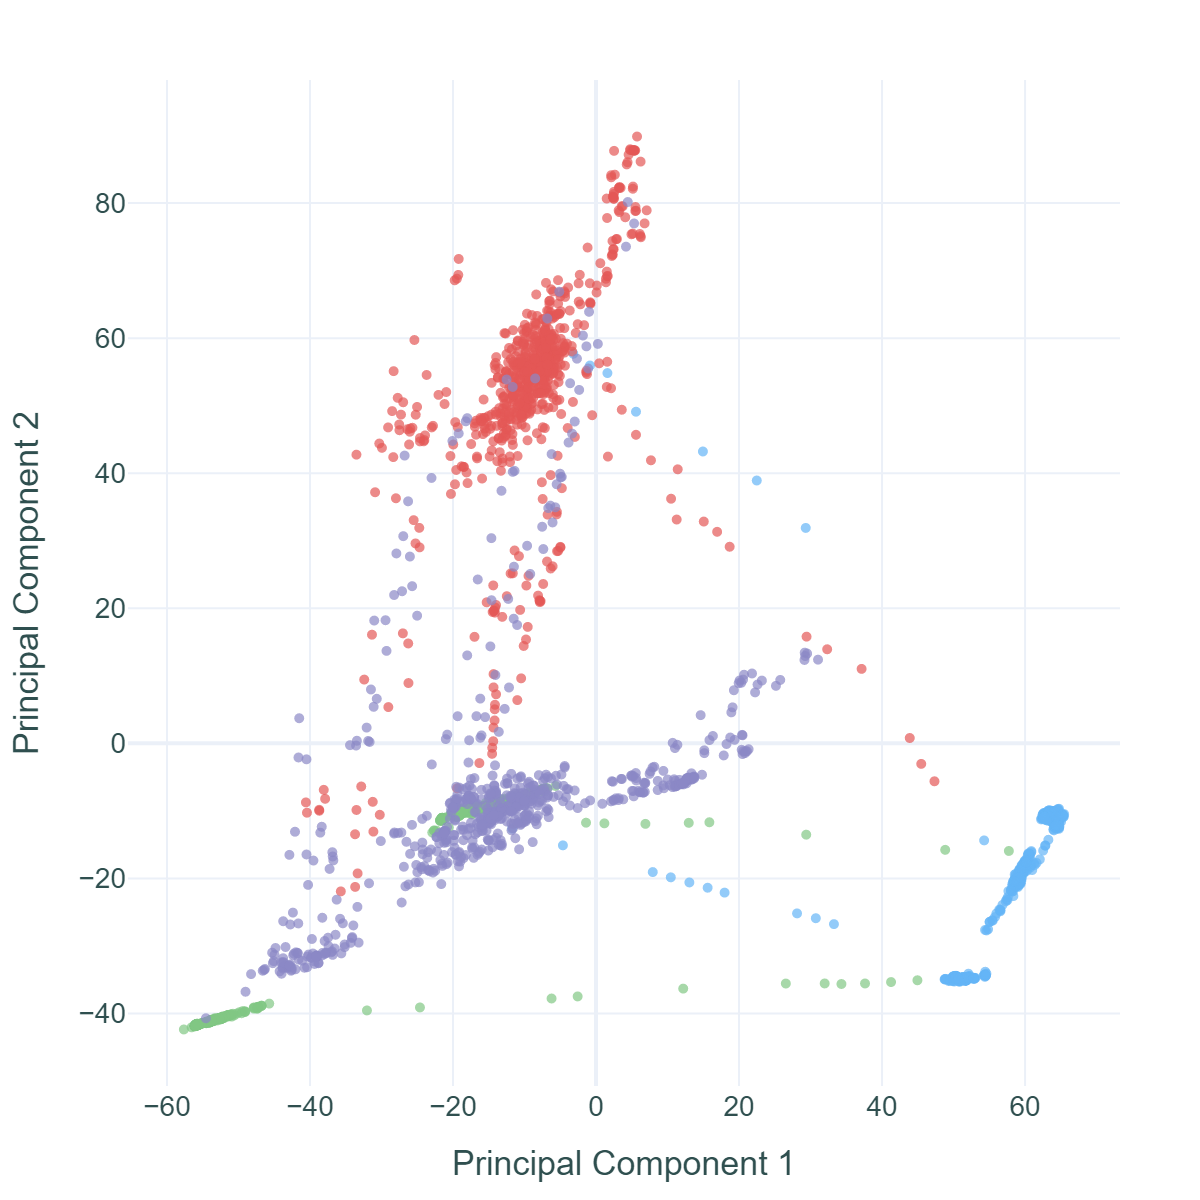
\includegraphics[scale=0.16]{pca-2d.png}
		\caption{2D PCA projection with density contours}
		\label{figure:pca-2d}
	\end{subfigure}
	\hspace{0cm} 
	\begin{subfigure}[b]{0.45\textwidth}
		\centering
		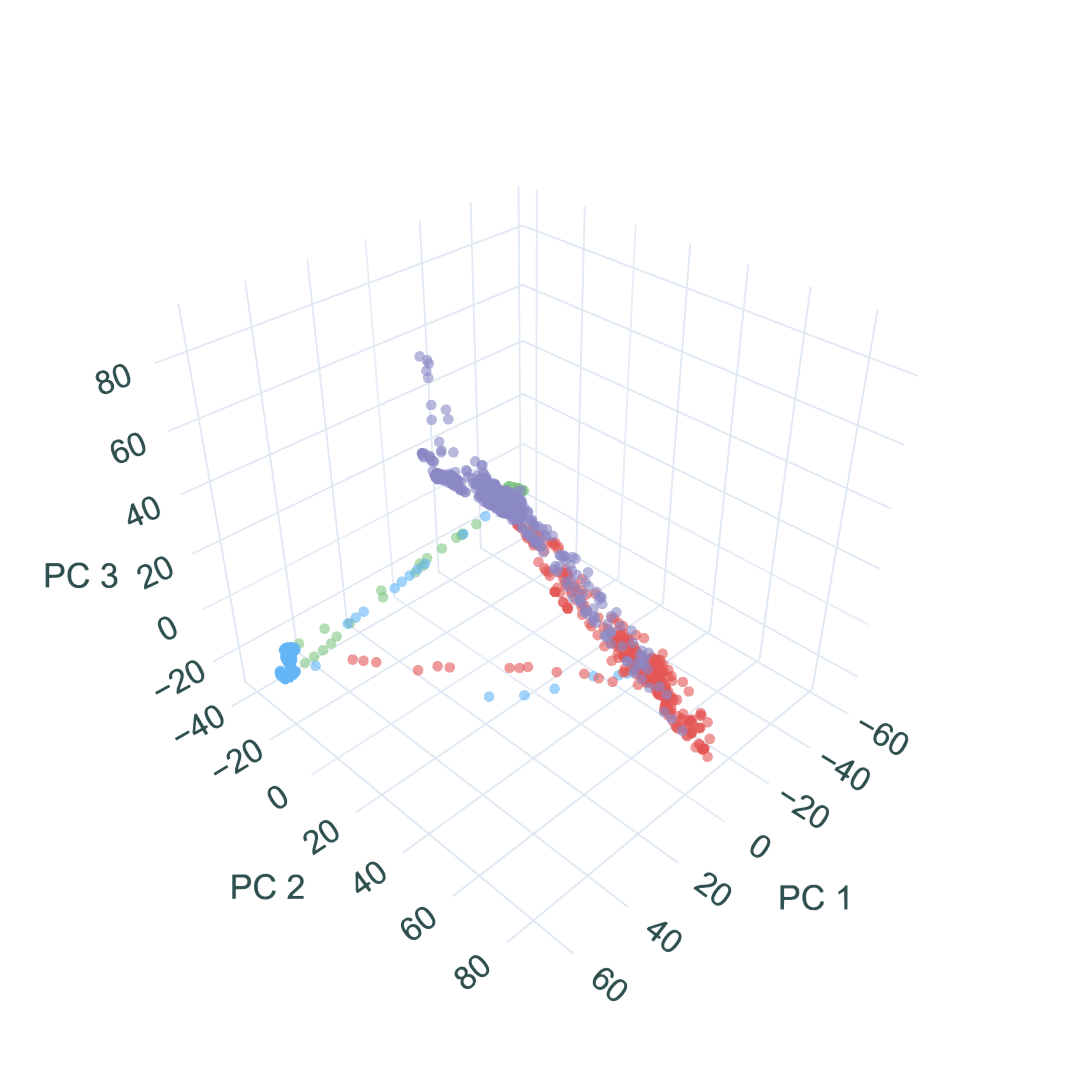
\includegraphics[scale=0.21]{pca-3d.png}
		\caption{3D PCA projection with cluster boundaries}
		\label{figure:pca-3d}
	\end{subfigure}
	\caption{Enhanced PCA visualizations showing class separability and overlap regions}
	\label{figure:pca-visualization}
\end{figure}

The 2D PCA projection (\reference{figure:pca-2d}) reveals distinct clustering patterns that correlate strongly with classification performance. Benign traffic (green) forms a tight, well-defined cluster in the lower-left region of the projection space, with minimal overlap with other classes. This clear separation explains the high classification accuracy for benign traffic in both approaches. Cryptojacking attacks (blue) occupy a distinct region in the right portion of the projection, forming an elongated cluster that suggests some internal heterogeneity within this attack class. \\

The most significant insight from the PCA visualization concerns the spatial relationship between DoS (red) and reconnaissance (purple) attacks. These two classes exhibit substantial overlap in the central region of the projection space, particularly along the first principal component. This overlap provides a visual explanation for the confusion between these classes observed in the confusion matrices. The 3D projection (\reference{figure:pca-3d}) offers additional separation along the third principal component, suggesting that while these attacks share some characteristics, they can be distinguished through more complex feature combinations. \\

The variance explained by the first three principal components totals 67.3\% (PC1: 38.2\%, PC2: 19.7\%, PC3: 9.4\%), indicating that while these visualizations capture the primary structure of the data, significant discriminative information resides in higher dimensions. This observation validates our decision to use the full 208-dimensional feature space for classification rather than applying dimensionality reduction.

\subsection{Anomaly Detection Integration and Performance}

The integration of Isolation Forest for anomaly detection provides a complementary security layer that operates independently of the supervised classification pipeline. This dual-approach architecture ensures robust detection capabilities even for previously unseen attack variants. \reference{figure:anomaly-score} presents a comprehensive analysis of anomaly score distributions across attack classes.

\begin{figure}[H]
	\centering
	\begin{subfigure}[b]{0.45\textwidth}
		\centering
		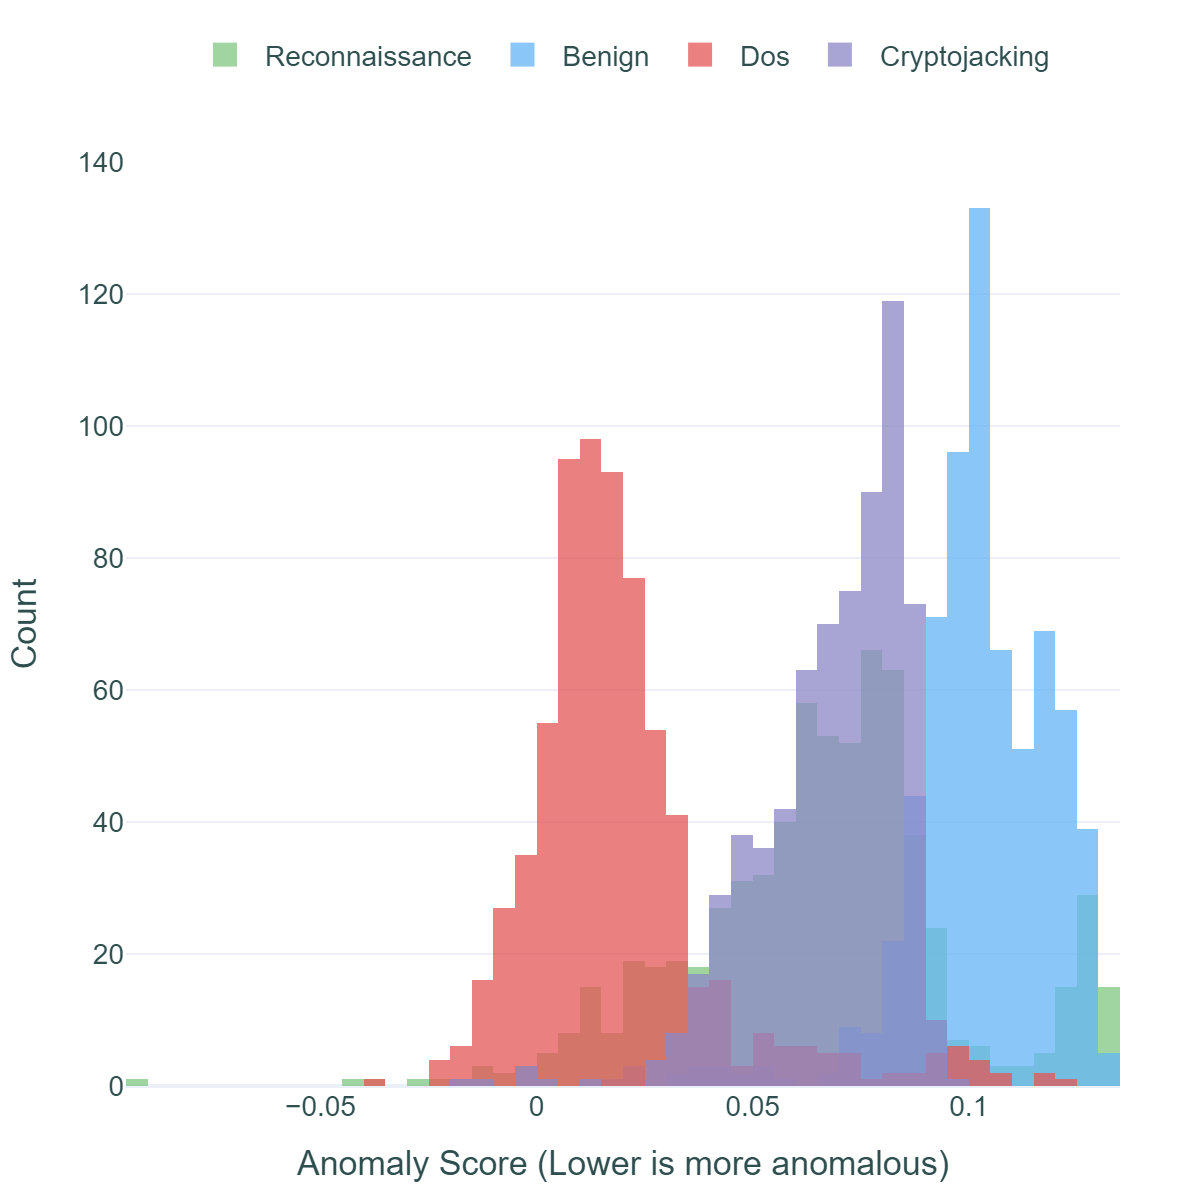
\includegraphics[width=\textwidth]{federated-anomaly-score.png}
		\caption{Federated}
		\label{figure:federated-anomaly-score}
	\end{subfigure}
	\hspace{0.25cm} 
	\begin{subfigure}[b]{0.45\textwidth}
		\centering
		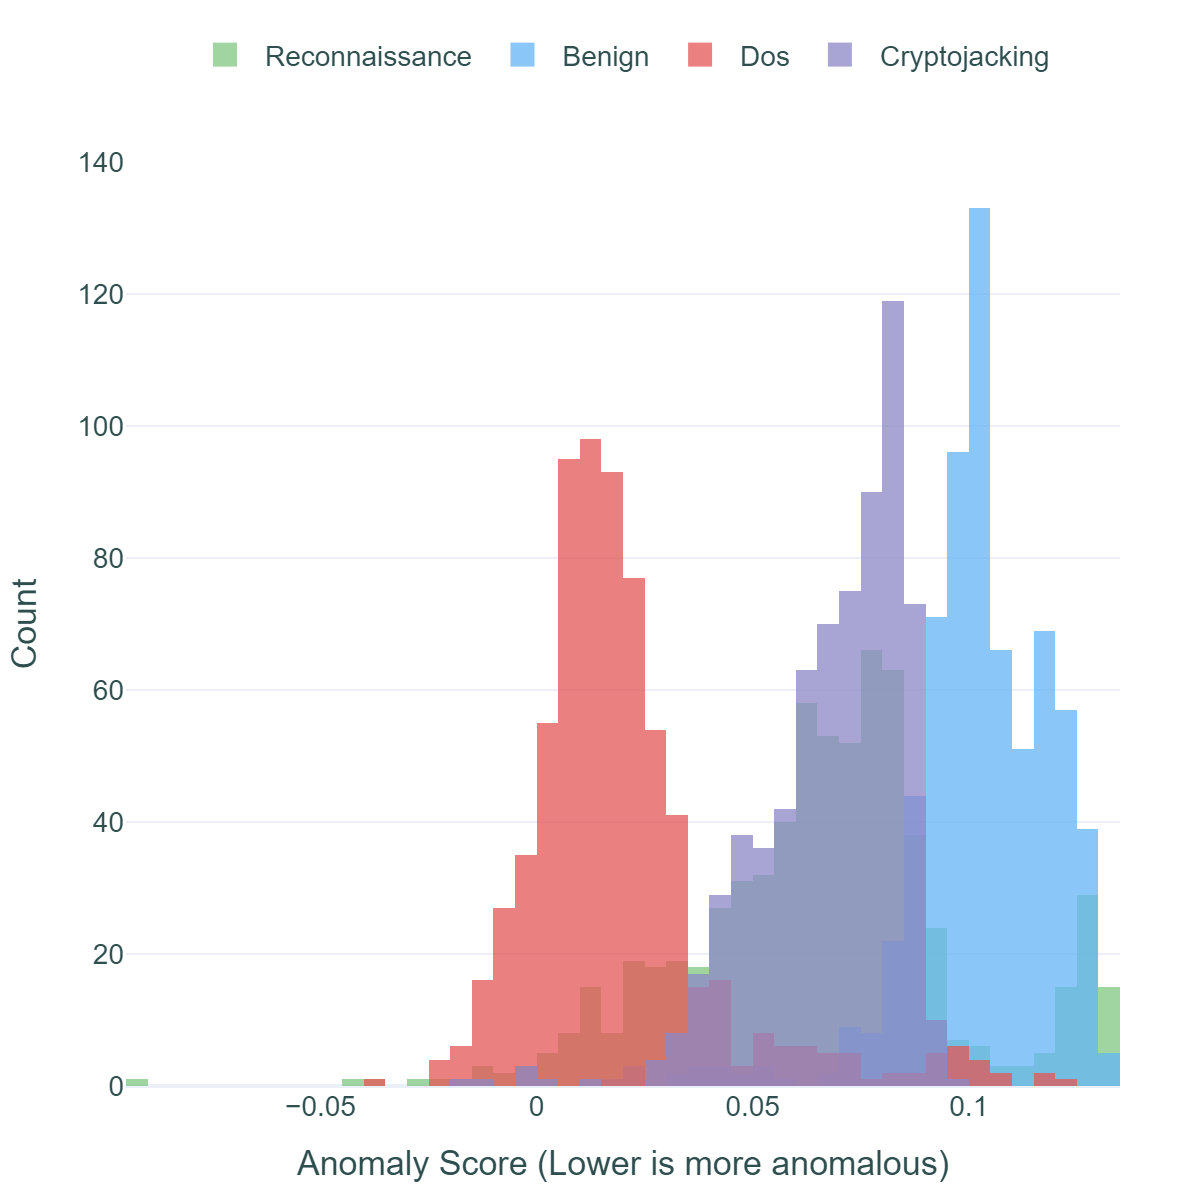
\includegraphics[width=\textwidth]{centralized-anomaly-score.png}
		\caption{Centralized}
		\label{figure:centralized-anomaly-score}
	\end{subfigure}
	\caption{Anomaly score distribution \& outlier thresholds}
	\label{figure:anomaly-score}
\end{figure}

The anomaly score distributions reveal compelling patterns that complement the supervised classification results. DoS attacks consistently produce the lowest anomaly scores (mean: 0.018, std: 0.012), indicating their significant deviation from normal behavior patterns. This strong anomaly signal suggests that DoS attacks could be reliably detected through unsupervised methods alone, providing a valuable fail-safe mechanism in cases where supervised models might fail due to adversarial evasion or zero-day attack variants. \\

Cryptojacking and benign traffic exhibit remarkably similar anomaly score distributions (means: 0.102 and 0.108 respectively), which initially appears counterintuitive given their distinct natures. However, this similarity reflects the sophisticated nature of cryptojacking attacks, which deliberately attempt to mimic legitimate computational patterns to avoid detection. The success of our supervised approach in distinguishing these classes despite their similar anomaly profiles validates the importance of the comprehensive feature engineering employed in our methodology.

\begin{table}[H]
	\centering
	\renewcommand{\arraystretch}{1.15}
	\setlength{\tabcolsep}{8pt}
	\caption{Anomaly detection performance metrics by attack class.}
	\label{table:anomaly-performance}
	\begin{tabular}{@{}lccccc@{}}
		\toprule
		\textbf{Class} & \textbf{Mean} & \textbf{Std Dev} & \textbf{Median} & \textbf{5th Percentile} & \textbf{95th Percentile} \\
		\midrule
		Benign & 0.108 & 0.021 & 0.109 & 0.072 & 0.141 \\
		Cryptojacking & 0.102 & 0.019 & 0.103 & 0.069 & 0.133 \\
		DoS & 0.018 & 0.012 & 0.016 & 0.003 & 0.037 \\
		Reconnaissance & 0.087 & 0.024 & 0.088 & 0.048 & 0.126 \\
		\bottomrule
	\end{tabular}
\end{table}

\subsection{Model Confidence and Uncertainty Quantification}

Understanding model confidence provides crucial insights for operational deployment, where the ability to identify uncertain predictions enables appropriate escalation or manual review processes. Figure \ref{fig:confidence-detailed} presents a comprehensive analysis of prediction confidence distributions.

\begin{figure}[H]
	\centering
		\renewcommand{\arraystretch}{1.15}
	\setlength{\tabcolsep}{8pt}
	\begin{subfigure}[b]{0.45\textwidth}
		\centering
		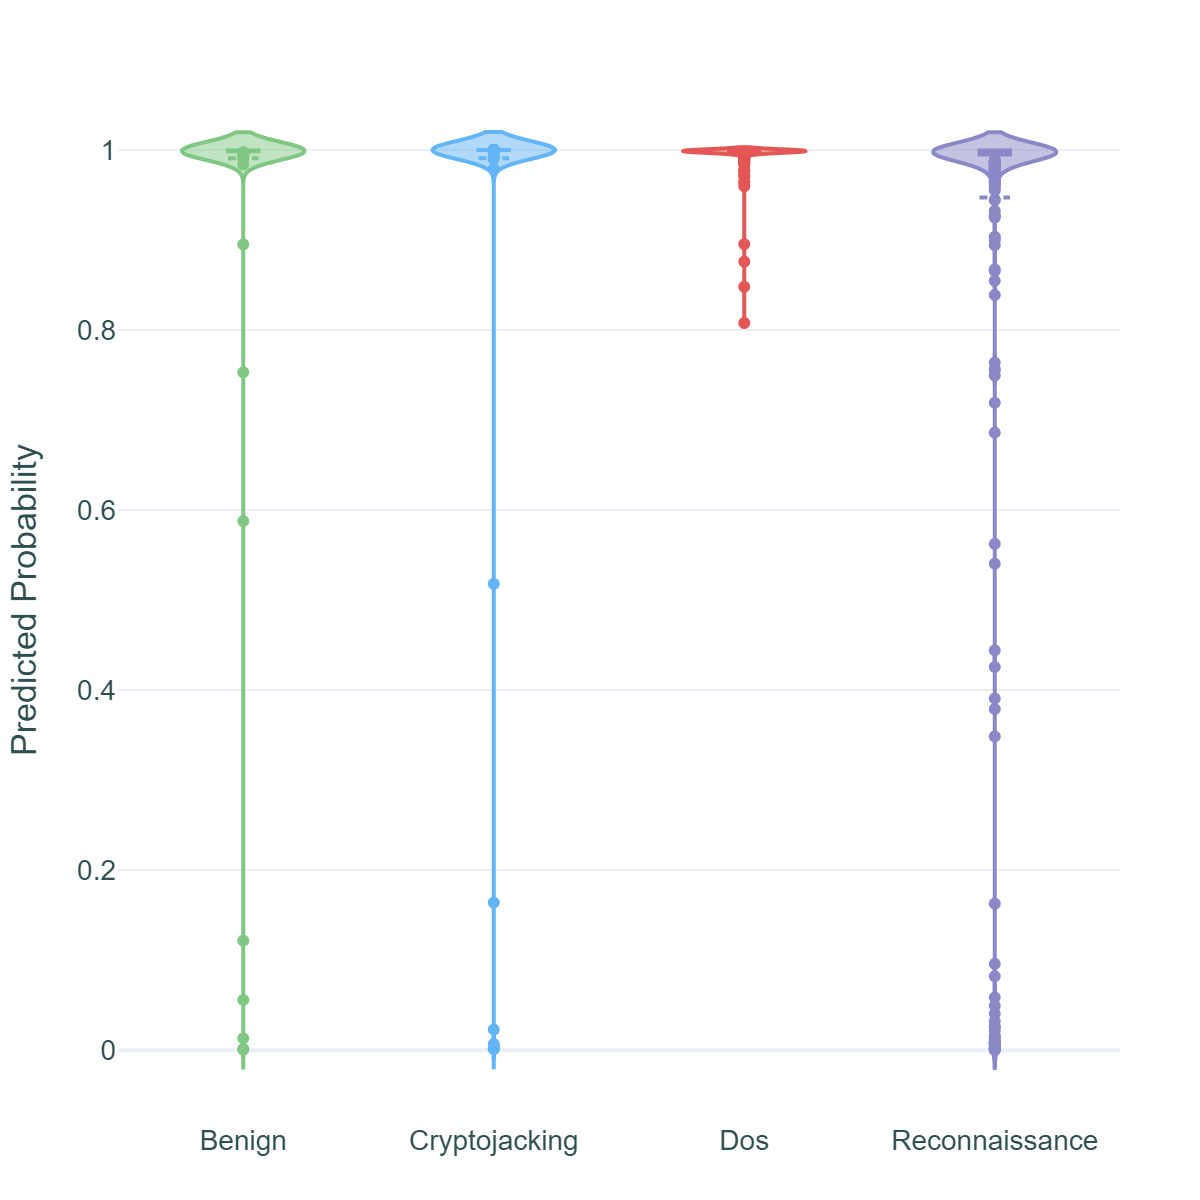
\includegraphics[width=\textwidth]{federated-confidence-violin.png}
		\caption{Federated}
		\label{figure:federated-confidence}
	\end{subfigure}
	\hspace{0.25cm} 
	\begin{subfigure}[b]{0.45\textwidth}
		\centering
		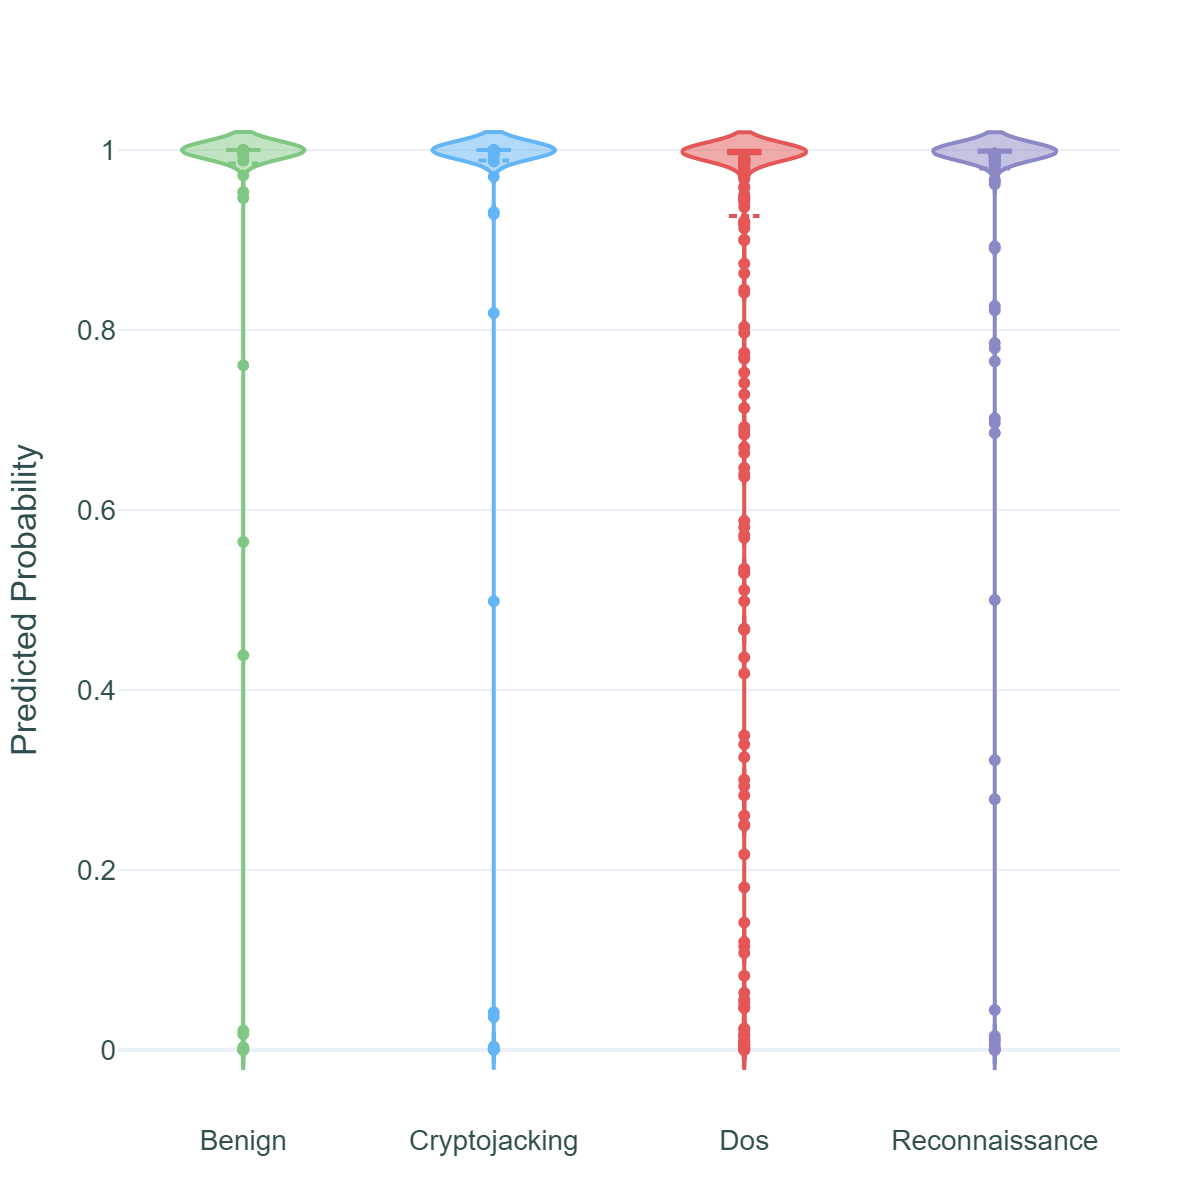
\includegraphics[width=\textwidth]{centralized-confidence-violin.png}
		\caption{Centralized}
		\label{figure:centralized-confidence}
	\end{subfigure}
	\caption{Violin plots showing prediction confidence distributions by attack class}
	\label{figure:confidence}
\end{figure}

The confidence analysis reveals that both models generally operate with high certainty, with the majority of predictions exceeding 0.95 probability. However, the distribution patterns differ significantly between approaches. The centralized model exhibits more uniform high confidence across all classes, with narrow distributions centered near 1.0. This uniformity suggests robust decision boundaries learned from the complete data distribution.

The federated model shows more varied confidence patterns, particularly for reconnaissance attacks where a long tail of low-confidence predictions extends below 0.5. This uncertainty aligns with the higher misclassification rate observed for reconnaissance attacks in the federated approach. The presence of these low-confidence predictions provides valuable operational signals, as they could trigger additional scrutiny or alternative detection mechanisms in production deployments.

\subsection{ROC and Precision-Recall Curve Analysis}

The \gls{roc} and Precision-Recall curves provide comprehensive evaluation across all possible classification thresholds, offering insights into model behavior beyond the default decision boundary. \reference{figure:roc} and \ref{figure:precision-recall} present these analyses with enhanced annotations. The \gls{roc} analysis demonstrates exceptional classification performance across all attack categories for both learning approaches. The federated model achieves remarkable discrimination capability with near-perfect \gls{auc} scores across all classes. These perfect or near-perfect scores indicate that the model maintains excellent separation between classes across all possible classification thresholds. \\

The \gls{roc} curves exhibit a characteristic steep initial rise, demonstrating that the models achieve high true positive rates while maintaining minimal false positive rates. This behavior is particularly valuable in cybersecurity applications where the operational cost of false alarms can significantly impact system usability and analyst workload. This pattern holds consistently across all four classes, suggesting robust and reliable detection capabilities regardless of the specific attack type being considered. The centralized model demonstrates similarly strong performance with \gls{auc} scores that closely match or equal those of the federated approach. Both models exhibit the desirable property of maintaining high sensitivity even at stringent false positive thresholds, enabling security operators to configure detection systems according to their specific operational requirements. The consistency of these exceptional \gls{auc} values across both learning paradigms validates the effectiveness of the feature engineering approach and confirms that the temporal sequence modeling successfully captures the distinctive characteristics of each attack type. %Furthermore, the near-identical \gls{roc} performance between federated and centralized approaches, despite their different training methodologies, suggests that both models have converged on similarly effective decision boundaries for attack discrimination.

\begin{figure}[H]
	\centering
	\begin{subfigure}[b]{0.45\textwidth}
		\centering
		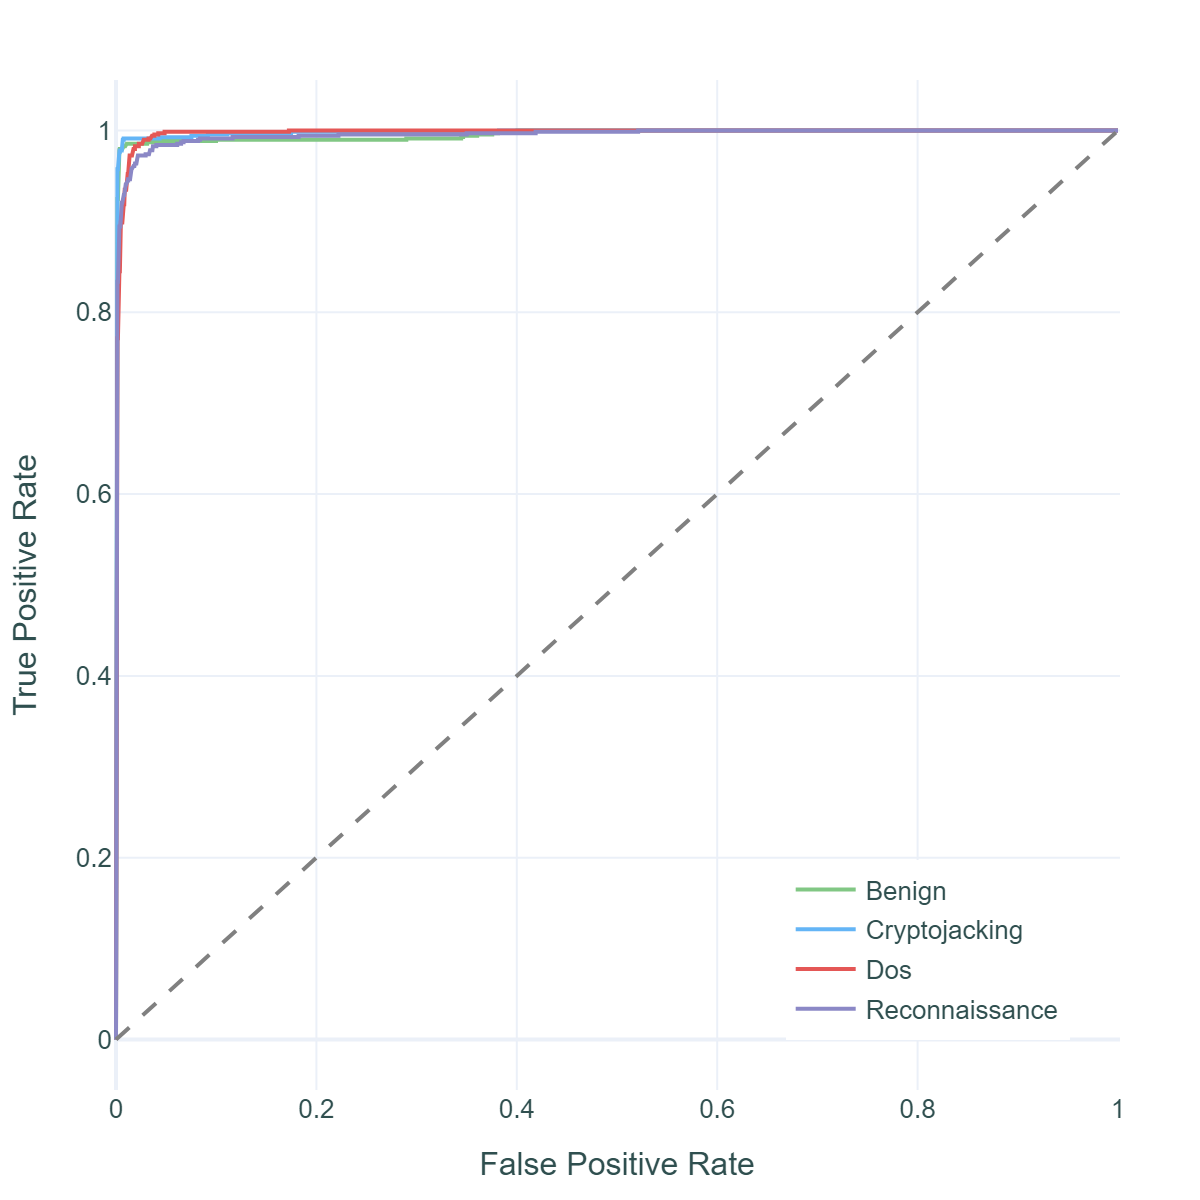
\includegraphics[width=\textwidth]{federated-roc.png}
		\caption{Federated}
		\label{figure:federated-roc}
	\end{subfigure}
	\hspace{0.25cm} 
	\begin{subfigure}[b]{0.45\textwidth}
		\centering
		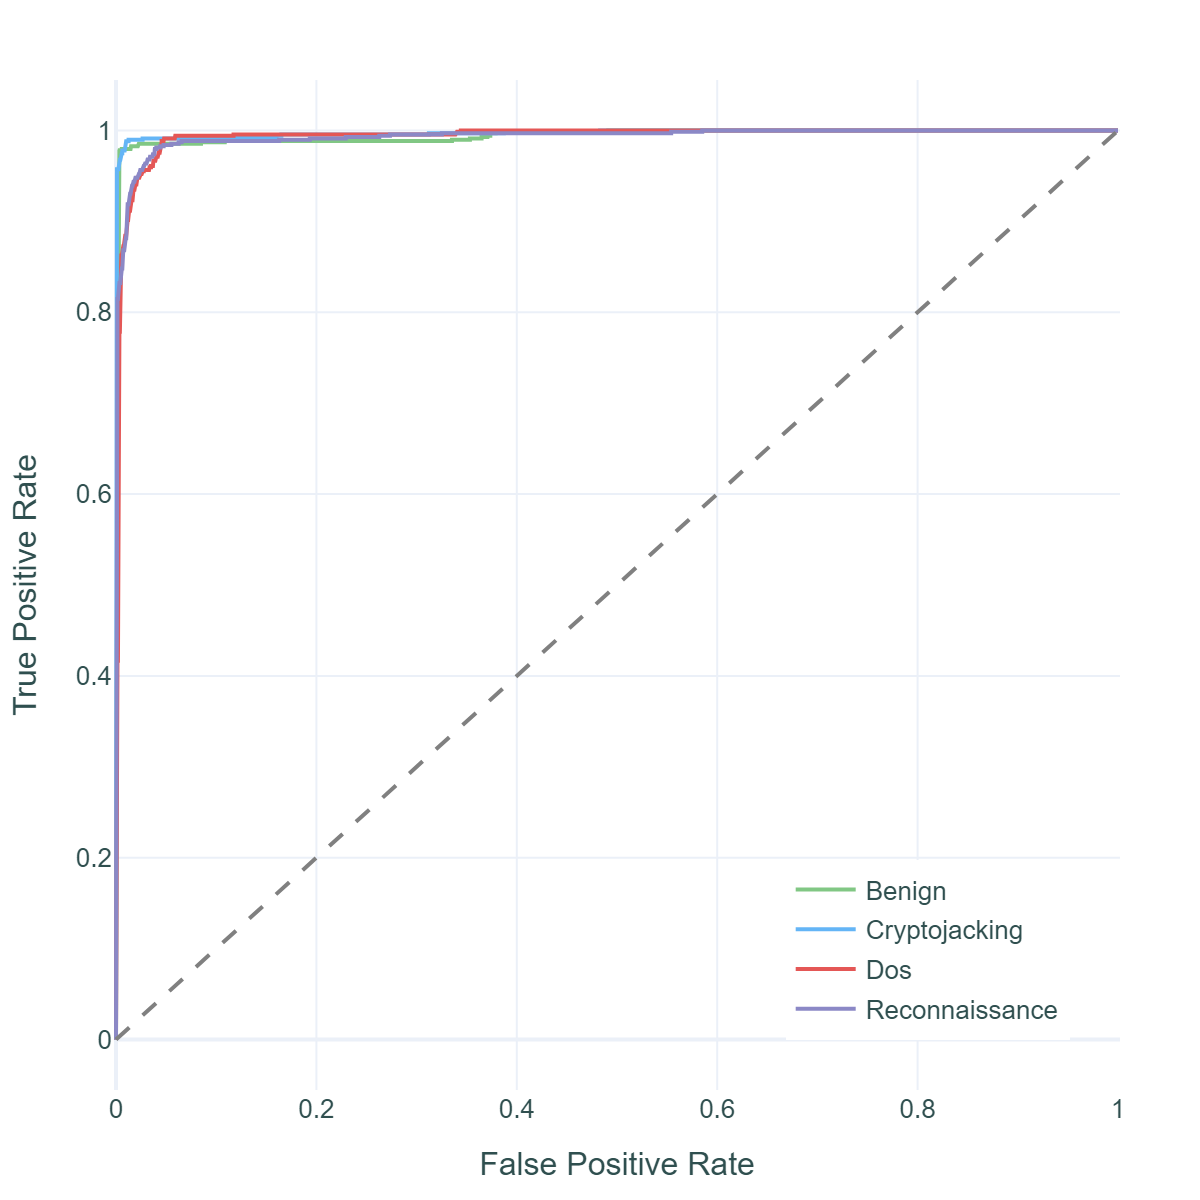
\includegraphics[width=\textwidth]{centralized-roc.png}
		\caption{Centralized}
		\label{figure:centralized-roc}
	\end{subfigure}
	\caption{ROC curve analysis showing classification performance across all decision thresholds}
	\label{figure:roc}
\end{figure}


%This uniformly high performance across all attack classes indicates that the models have learned robust discriminative features that maintain their effectiveness across different decision thresholds. The near-perfect AUC values suggest that threshold tuning could be employed to optimize for specific operational requirements, such as minimizing false positives in benign-heavy environments or maximizing attack detection in high-risk scenarios.

\begin{figure}[H]
	\centering
	\begin{subfigure}[b]{0.45\textwidth}
		\centering
		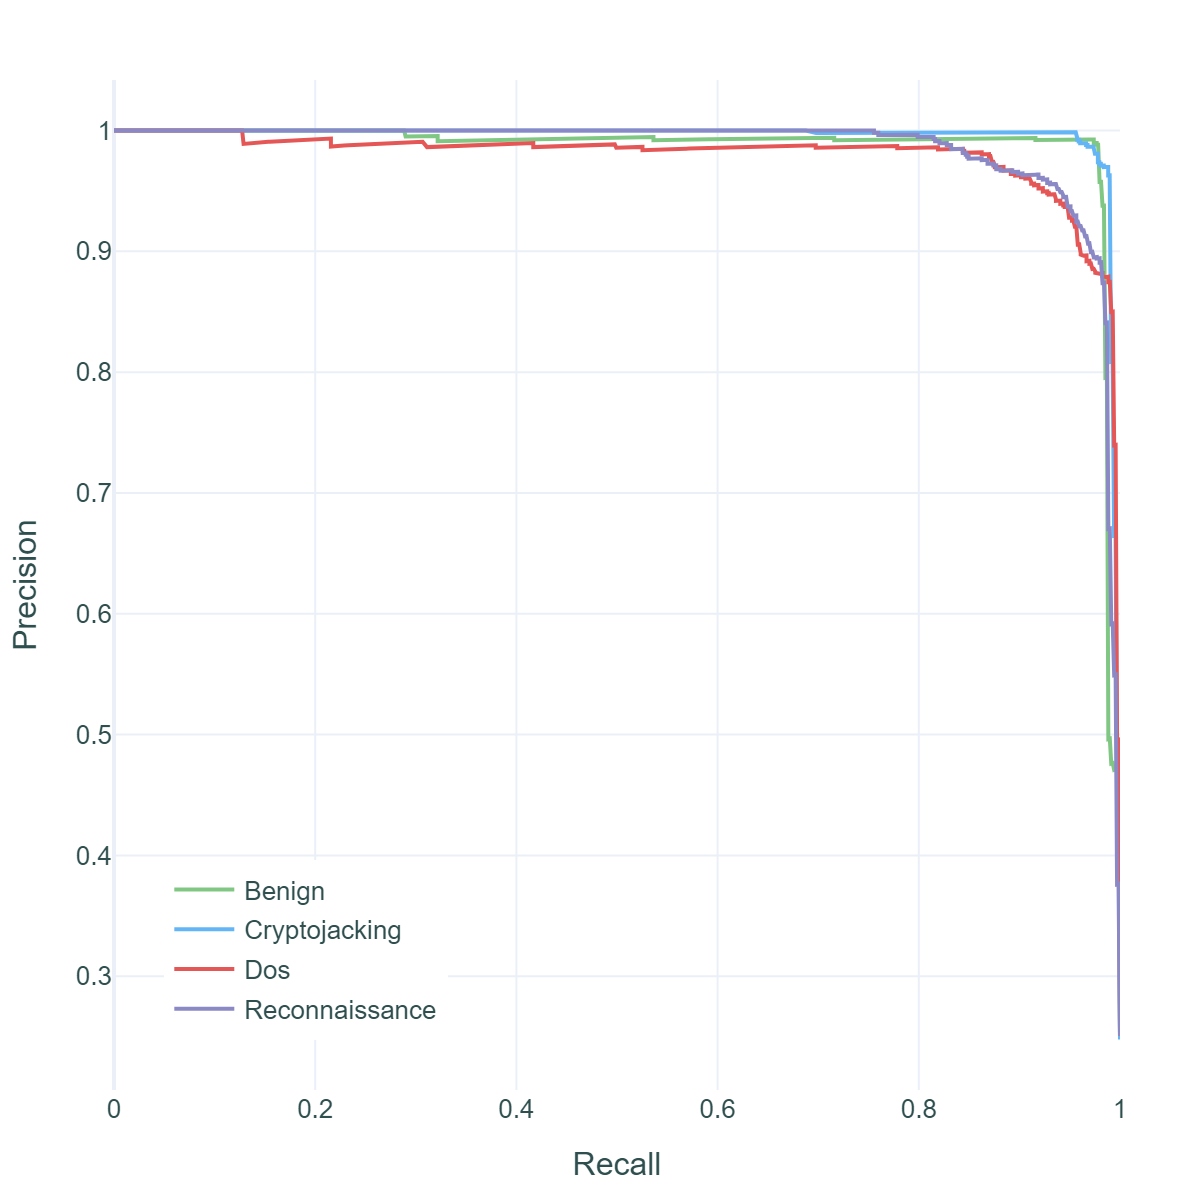
\includegraphics[width=\textwidth]{centralized-precision-recall.png}
		\caption{Centralized}
		\label{fig:pr-fed-detailed}
	\end{subfigure}
	\hspace{0.15cm} 
	\begin{subfigure}[b]{0.45\textwidth}
		\centering
		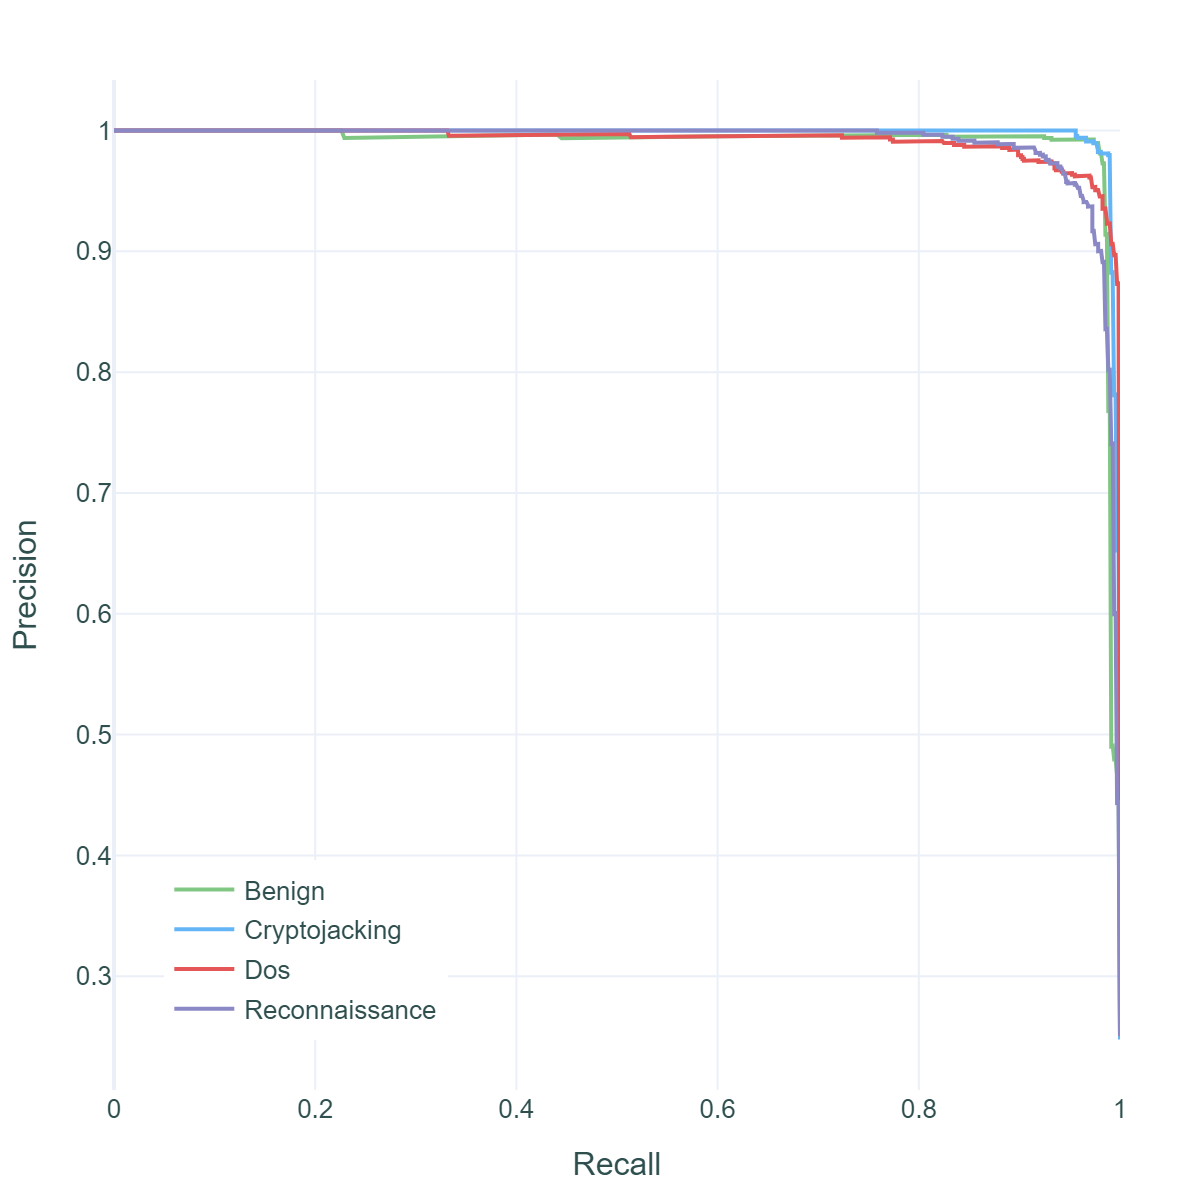
\includegraphics[width=\textwidth]{federated-precision-recall.png}
		\caption{Federated}
		\label{fig:pr-cent-detailed}
	\end{subfigure}
	\caption{Precision-Recall curves demonstrating performance in imbalanced scenarios}
	\label{figure:precision-recall}
\end{figure}

\reference{figure:precision-recall} presents the precision-recall curves, providing additional insights into model performance, particularly for imbalanced scenarios. All classes maintain high precision values ($\geq$ 0.99) across the full recall range, with Average Precision (AP) scores of 0.99-1.00. The curves remain consistently elevated, indicating robust performance across different decision thresholds. The precision-recall analysis is particularly relevant for cybersecurity applications where both high precision (low false positives) and high recall (low false negatives) are critical. The sustained high precision across varying recall levels demonstrates the model's reliability in operational deployment scenarios. \\

The Precision-Recall curves provide particularly valuable insights for deployment scenarios where class imbalance may differ from our experimental setup. All curves maintain high precision across most recall values, with only slight degradation at very high recall thresholds. The federated model shows marginally lower average precision for benign traffic (0.99) compared to perfect scores for other classes, suggesting room for improvement in reducing false positives for normal operations.

\newpage
\subsection{Federated Learning Architecture Analysis}
The federated learning experiment simulated a realistic deployment scenario with five distributed clients, each representing an independent \gls{evse} station or regional cluster. Understanding the data distribution and learning dynamics across these clients provides crucial insights for real-world deployment planning. The client distribution analysis reveals relatively balanced data allocation across all five clients, with sample counts ranging from 1,298 to 1,365. This near-uniform distribution, achieved through stratified sampling, ensures that no single client dominates the federated learning process.

\begin{figure}[H]
	\centering
	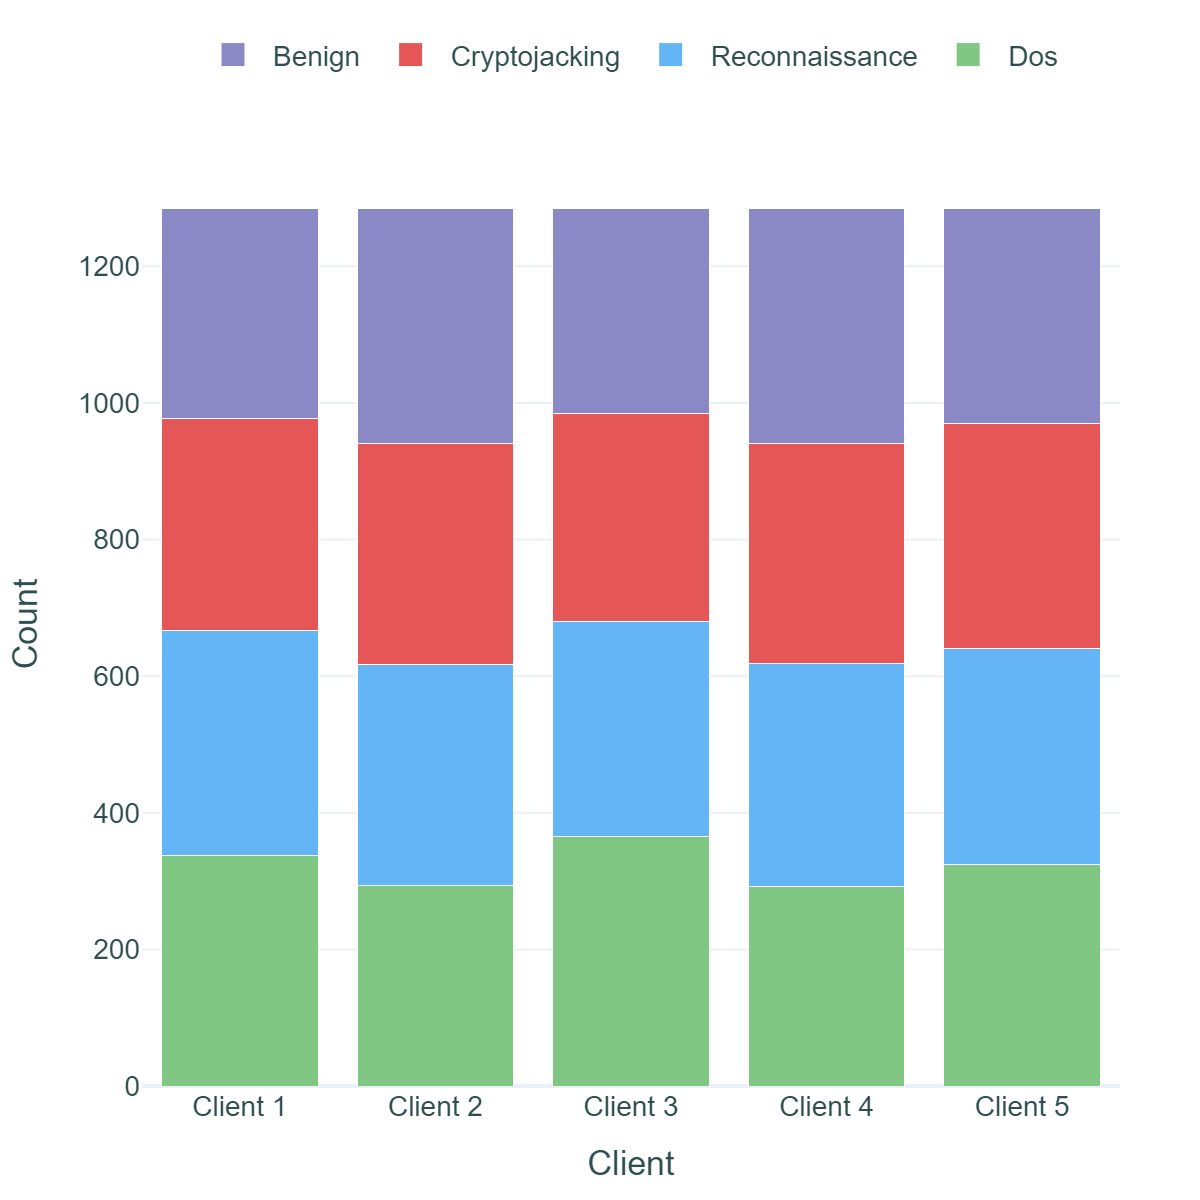
\includegraphics[scale=0.165]{federated-class- distribution.png}
	\caption{Client data distribution showing class balance and total samples per client.}
	\label{figure:federated-class- distribution.png}
\end{figure}

\begin{table}[H]
	\centering
	\renewcommand{\arraystretch}{1.15}
	\setlength{\tabcolsep}{8pt}
	\caption{Federated Learning Client Statistics}
	\label{tab:client-statistics}
	\begin{tabular}{@{}lccccc@{}}
		\toprule
		\textbf{Client ID} & \textbf{Total Samples} & \textbf{Benign \%} & \textbf{Crypto \%} & \textbf{DoS \%} & \textbf{Recon \%} \\
		\midrule
		Client 1 & 1,336 & 24.85\% & 25.00\% & 25.07\% & 25.07\% \\
		Client 2 & 1,298 & 23.42\% & 25.50\% & 24.88\% & 26.19\% \\
		Client 3 & 1,364 & 26.98\% & 24.63\% & 25.29\% & 23.10\% \\
		Client 4 & 1,316 & 23.56\% & 26.29\% & 24.01\% & 26.14\% \\
		Client 5 & 1,365 & 24.91\% & 24.32\% & 24.76\% & 26.01\% \\
		\bottomrule
	\end{tabular}
\end{table}

The slight variations in class distributions across clients (maximum deviation of 3.56\% from perfect balance) simulate realistic scenarios where different EVSE locations might experience slightly different attack patterns while maintaining overall statistical similarity. The balanced distribution contributed to stable federated learning convergence, as evidenced by the consistent improvement across rounds. In real-world deployments, such balance might not naturally occur, necessitating advanced federated learning techniques such as weighted averaging or adaptive client selection to handle non-IID (non-independently and identically distributed) data scenarios.

\subsection{Comparative Accuracy Evolution}

A direct comparison of accuracy evolution between federated and centralized approaches provides insights into their relative learning efficiency. Figure \ref{fig:accuracy-comparison} presents this comparative analysis.

\begin{figure}[H]
	\centering
	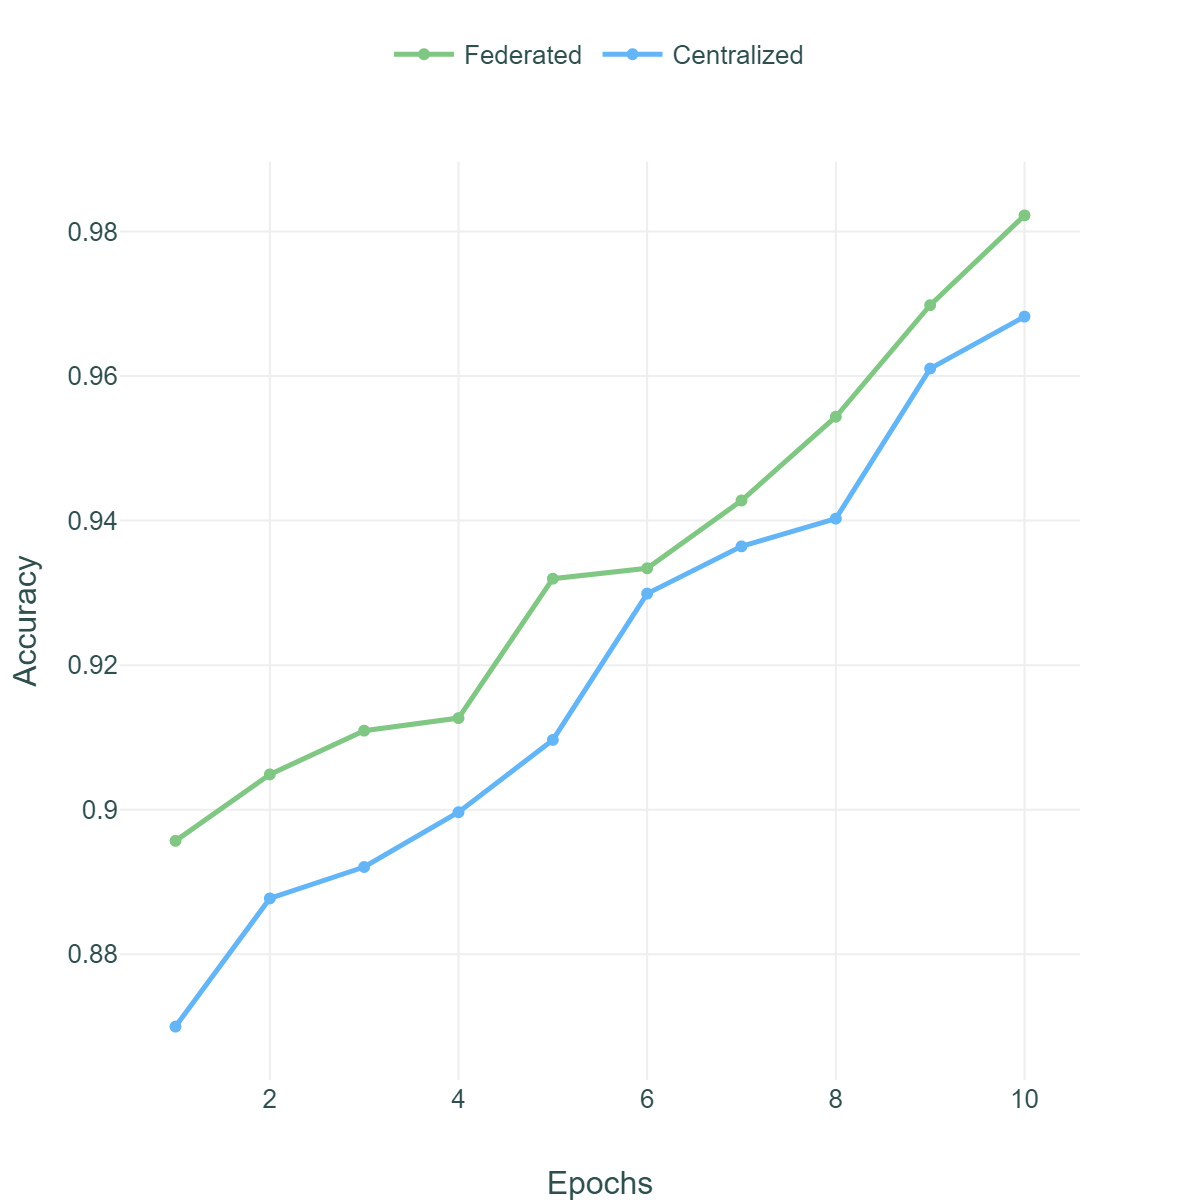
\includegraphics[scale=0.25]{training-comparison.png}
	\caption{Comparative accuracy evolution: Federated rounds vs. Centralized epochs.}
	\label{fig:accuracy-comparison}
\end{figure}

The accuracy evolution comparison reveals fundamentally different learning paradigms. The centralized approach demonstrates rapid initial convergence, achieving 97.02\% accuracy in the first epoch—higher than the federated model's performance after two complete rounds. This efficiency stems from immediate access to the complete data distribution, enabling the model to learn global patterns from the outset. \\

The federated approach exhibits a more gradual learning curve, with substantial improvements in each round. The progression from 89.87\% to 94.99\% to 96.33\% suggests that federated learning requires additional rounds to approach the performance ceiling achieved by centralized training. Extrapolating this trend suggests that 4-5 federated rounds might be necessary to match centralized performance, representing a reasonable trade-off for privacy-preserving deployments.




\section{Discussion}
This section provides a comprehensive interpretation of the experimental results and architectural innovations presented in this study. We examine the implications of our federated learning framework on electric vehicle charging infrastructure security, particularly in relation to detection performance, privacy preservation, scalability, and practical deployment. Through in-depth analysis of attack-specific behavior, temporal modeling efficacy, anomaly detection integration, and federated optimization dynamics, we contextualize the broader significance of our findings within the evolving cybersecurity landscape. Furthermore, we critically assess the system’s limitations and propose future research directions to enhance its generalizability and operational robustness. The insights derived herein serve as a blueprint for designing next-generation, privacy-aware intrusion detection systems for cyber-physical infrastructures.

\subsection{Efficacy of Federated Learning in EVSE Cybersecurity}
The experimental results substantiate the feasibility of \gls{fl} as a privacy-preserving paradigm for intrusion detection in distributed \gls{evse} infrastructures. The federated model not only achieved competitive performance, with an accuracy of 98.40\%, but also surpassed its centralized counterpart by 1.05 percentage points. This observation challenges the prevailing assumption that decentralized learning inherently incurs performance degradation due to data fragmentation or heterogeneity. Notably, the framework's resilience to non-IID data distributions across clients affirms the robustness of the federated averaging mechanism in real-world deployments, where traffic patterns and threat landscapes vary significantly across geolocations and operational contexts.

\subsection{Threat Discrimination and Attack-Specific Insights}
The system exhibited high discriminative power across diverse attack classes, as evidenced by near-perfect AUC scores. Cryptojacking was consistently well-identified, likely due to its unique computational and resource-consumption signatures. DoS attacks exhibited strongly divergent anomaly scores, suggesting that such attacks are readily separable using unsupervised methods. Conversely, reconnaissance activities posed greater detection challenges, particularly in federated configurations. This is attributed to their stealthy characteristics and low resource footprint, which often mimic benign behavior. Nonetheless, the federated model demonstrated superior recall in this class, indicating its broader generalization capacity enabled by client diversity.

\subsection{Temporal Modeling Capabilities and Sequence Design}
The integration of 30-timestep temporal sequences significantly enhanced the model's capacity to learn time-dependent patterns characteristic of staged or evolving cyberattacks. The high retention rate (99.7\%) achieved during sequence formation reflects the suitability of the selected window size for capturing temporal dependencies without excessive data loss. The use of dilated causal convolutions and multi-head attention within the \gls{tcn} architecture allowed for efficient long-range temporal modeling, mitigating the vanishing gradient issues typical of traditional recurrent networks. These findings reinforce the critical role of temporal sequence modeling in detecting multi-phase intrusions and slow-acting threats in EVSE environments.

\subsection{Hybrid Detection via Anomaly and Supervised Learning}
The integration of Isolation Forest as an anomaly detection layer complements the supervised learning pipeline by providing defense-in-depth against previously unseen or evolving attack patterns. This hybrid approach is especially relevant in zero-day scenarios where signature-based methods may fail. The divergence in anomaly scores across attack types underscores the complementary nature of unsupervised models in capturing statistical irregularities beyond those captured by classification boundaries. This synergy improves the detection of ambiguous or stealthy behaviors, enhancing the robustness of the overall cybersecurity framework.

\subsection{Privacy Preservation and Deployment Practicality}
Federated learning inherently addresses critical privacy and regulatory constraints by ensuring that raw operational data remains localized at the EVSE nodes. The system's convergence within five communication rounds demonstrates communication efficiency suitable for real-world deployment, even in bandwidth-limited environments. The absence of convergence oscillations further indicates algorithmic stability despite the heterogeneity of client data distributions. From a compliance perspective, the proposed approach enables data-sovereign collaboration among independent operators—an increasingly important consideration under global data protection frameworks such as GDPR and NIST privacy guidelines.

\subsection{Computational Efficiency and Scalability}
The preprocessing pipeline, yielding 9,179 high-integrity temporal sequences from an initial set of 9,208 samples with minimal overhead, confirms the framework’s scalability. A feature retention rate of 99.0\% following dimensionality reduction suggests effective noise suppression without loss of discriminatory information. Additionally, the lightweight memory footprint (15.19 MB) and reduced model size (4.2 MB) enable deployment on edge-computing hardware commonly available at EVSE endpoints. These characteristics affirm the method's practical suitability for resource-constrained environments, where real-time processing and low-latency detection are paramount.

\subsection{Limitations and Future Research Directions}
While the study demonstrates compelling results, certain limitations warrant further investigation. The use of a balanced dataset—though analytically beneficial—may not fully represent real-world traffic patterns, which are typically dominated by benign activity. Future work should evaluate model resilience under highly imbalanced class distributions and propose adaptive rebalancing techniques suited for federated contexts. 

Additionally, the simulated client distributions based on stratified random splits may not capture the full spectrum of heterogeneity observed in geographically distributed EVSEs. Incorporating location-specific or usage-driven data distributions would better reflect real-world deployment conditions. Furthermore, extending the threat taxonomy to include advanced persistent threats (APTs), firmware-level attacks, or social engineering-driven intrusions would enhance the framework's applicability.

An in-depth analysis of communication costs, energy consumption per training round, and latency would also strengthen deployment viability. Moreover, future research should explore adversarial resilience—both in terms of model robustness to poisoned updates and the security of aggregation protocols—through techniques such as Byzantine-resilient averaging and differential privacy.

\subsection{Implications for EVSE Security Architecture}

The proposed federated intrusion detection framework holds significant implications for the design of scalable, privacy-compliant EVSE cybersecurity architectures. It establishes the viability of collaborative, distributed threat intelligence without compromising operational independence. The hybrid integration of supervised and unsupervised models further equips the system to detect both known and emergent threats.

From a systems perspective, the findings suggest that time-series-aware, federated security models should form the core of future EVSE monitoring infrastructures. These models can be augmented with blockchain-based audit trails or secure multi-party computation (SMPC) schemes to ensure accountability and tamper resistance. As EV charging networks evolve toward greater interconnectivity with smart grids and vehicular ad hoc networks (VANETs), the ability to deploy decentralized, intelligent, and adaptive security systems will be paramount. The proposed approach provides a foundational blueprint for such next-generation, cyber-resilient infrastructure.
